\subsection{First structure notes}
\subsubsection{Overlap of different models}
\begin{itemize}
    \item High overlap of top eigenspace of different models
    \item The peak of the overlap for layerwise eigenspace happens at dimension $n$, where $n$ is the number of output channels for convolutional layers and the number of output neurons for FC layers.
    \item Assumptions: The reason is that the gram matrix of the input of the layer is close to rank 1. For FC layers, it has been shown that $\E[\vx \vx^T]$ is close to rank 1.
    \item For convolutional layers, we have also observed that $\E[\mX \mX]^T]$ is close to rank 1, where $X$ is a matrix transformed from the input according to the modular hessian paper.
    \item The connections are still unclear and require more investigations.
\end{itemize}

\subsubsection{Kronecker product decomposition of Hessians for FC layers}
\begin{itemize}
    \item For FC networks, we can then express the weight hessian block w.r.t. the $p$-th and $q$-th layer in the form of $$\mH_{\vw^{(p)}\vw^{(q)}} l = \mU^{(p)T}\mA\mU^{(q)} \otimes \vx^{(p)}\vx^{(q)T}.$$
    \item We focus on Hessians with respect to a single layer. For a fixed layer $p$ if there is no confusion, we write
    $$\mH_{\vw\vw} l = \nabla_\vw^2 l = \mM \otimes \vx\vx^T.$$
    \item Show the approximation is good for top eigenvalues and top eigenspace.
    \item Assumption: The approximation is actually for $\mG_0+\mG_1+\mG_2$ in the paper (or $\mG_0+\mG_1$).
    \item Similar hierarchy structure in $\mM$ and/or $\vx\vx^T$. We can probably tSNE to observe the clustering in $\mM$ and/or $\vx\vx^T$.
\end{itemize}

\subsubsection{Random Label}
\begin{itemize}
    \item The disappearance of the gap between top $C$ eigenvalues and the bulk for random labels.
    \item Experiment on whether the top $C^2$ eigenvalues still exist (i.e. seperation between $\mG_2$ and $\mG_3$.
    \item Observe the clustering in $\Delta$ in the paper and $\mM$.
    \item Explain why Kronecker decomposition is still a good decomposition.
\end{itemize}

\subsection{Structure of \texorpdfstring{\E[\mM]}{EM}}
\ynote{Probably need more analysis on why the approximate is good.}

\snote{Clustering analysis on $\Delta$ matrices, maybe some provable claims on the initialization?
Observations for random label cases and corresponding explainations.}

\subsection{Structure of Output Hessian \texorpdfstring{$\E[\mM]$}{EM}}
\label{sec:struct_M}
\begin{figure}[th]
    \centering
    \begin{subfigure}[b]{0.32\textwidth}
        \centering
        \captionsetup{justification=centering}
        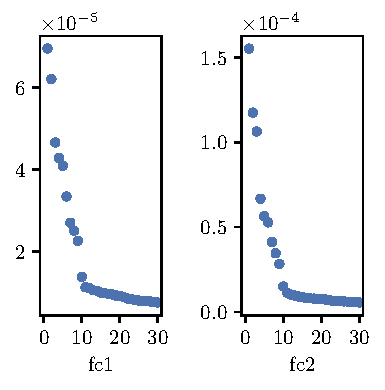
\includegraphics[width=\textwidth]{Figures/Eigenspectrum/UTAU/UTAU_sigval_d30_CIFAR10_Exp1_LeNet5_fixlr0.01R1_E-1_fc1fc2.pdf}
        \caption{Minimum}
        \label{fig:UTAU_spec_minima}
    \end{subfigure}\hfill
    \begin{subfigure}[b]{0.32\textwidth}
        \centering
        \captionsetup{justification=centering}
        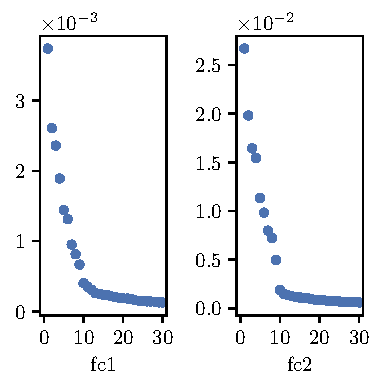
\includegraphics[width=\textwidth]{Figures/Eigenspectrum/UTAU/UTAU_sigval_d30_CIFAR10_Exp1_LeNet5_fixlr0.01R1_E0_fc1fc2.pdf}
        \caption{Random Initialization}
        \label{fig:UTAU_spec_init}
    \end{subfigure}\hfill
    \begin{subfigure}[b]{0.32\textwidth}
        \centering
        \captionsetup{justification=centering}
        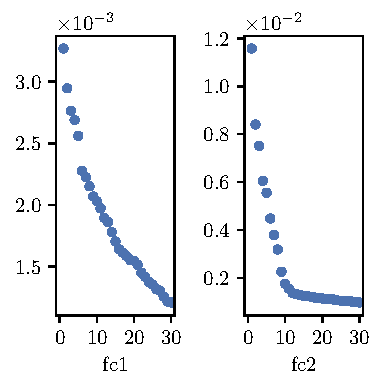
\includegraphics[width=\textwidth]{Figures/Eigenspectrum/UTAU/UTAU_sigval_d30_CIFAR10_RandomLabel_LeNet5_fixlr0.01_RLR1_E-1_fc1fc2.pdf}
        \caption{Minimum (Random Label)}
        \label{fig:UTAU_spec_RL}
    \end{subfigure}
    \captionsetup{justification=centering}
    \caption{Eigenspace overlap between models}
    \label{fig:UTAU_spec}
\end{figure}

\cref{fig:UTAU_spec_minima} and \cref{fig:UTAU_spec_init} shows the eigenspectrum of $\E[\mM]$ for FC2 networks at minimum and at initialization. In both cases we can see there are 9 or 10 outliers in the eigenspectrum. This phenomenon does not appear for dataset with random labels as shown in \cref{fig:UTAU_spec_RL}. Similar results are observed for other networks.

Gaps in eigenvalue distribution around dimension 10 are also observed in the eigenspectrum of full Hessians, agreeing with previous empirical studies. \citet{sagun2017empirical} suggests that there is a gap in Hessian eigenvalue distribution around the number of classes $C$ in most cases, where $C=10$ in our case. We conjecture this phenomenon is closely related to the structure of $\E[\mM]$ and will discuss more in \cref{sec:emp_outlier}.

\citet{papyan2019measurements} provides explanation for the gap in eigenspectrum using class clustering. Although we reproduced their results on their networks, there is no clear class clustering for both $\E[M]$ and layerwise Hessian at the Minimum for networks we experiment on. The reason is unclear but we conjecture that class clustering is only significant for very large networks.

The outliers at initialization, however, is easy to explain. Similar to \citet{papyan2019measurements} suggests for full Hessian, we observe logit clustering in $\E[\mM]$'s. Since there are $C$ logits, we would expect there are $C$ outliers. The results are shown in Appendix.

\subsection{Explanation for eigenspace overlap}
Moreover, since the neurons can be permuted to give equivalent models while changing eigenvectors, we can assume that eigenvectors of $\E[\mM]_1$ and $\E[\mM]_2$ have no correlation and thus have an expected inner product of $\frac{1}{\sqrt{n}}$. Thus, $\Overlap(\mV_1, \mV_2) =\frac{1}{k}\|\mV_1^T\mV_2\|^2_F = \frac{k}{n}$ and the overlap of top $k$ eigenspace of the true Hessian would be approximately $\frac{k}{n}(\hE[\vx]_1 \cdot \hE[\vx]_2)^2$. \ynote{Any further evidence/proof required?} In addition, for the first layer, models with the same dataset would have the same $\hE[\vx]$, and that would lead to an overlap close to 1 at dimension $n$.

Then, consider the $(n+1)$-th eigenvector of the first model $\vv_1$, since the top $n$ eigenvectors already span the full subspace $\mI_n \otimes \hE[\vx]_1$, $\vv_1$ will be orthogonal to this subspace. If $\hE[\vx]_1 \cdot \hE[\vx]_2$ is large, as we will shown empirically, $\vv_1$ will also be approximately orthogonal to $\mI_n \otimes \hE[\vx]_2$. The same applies to the $(n+1)$-th eigenvector of the second model, $\vv_2$. Then, again due to neuron permutation, we expect that $\vv_1 \cdot \vv_2$ is small. Thus, the overlap of the dimension $(n+1)$ eigenspace will decrease immediately and we will see a peak at dimension $n$. \ynote{Can there be a better/shorter explanation or just omit the explanation for the peak at dimension $n$?}

Indeed, we observe this phenomenon in () as shown in Fig. 4.4. In addition, the peak at dimension $n$ is high for all the layers. This would suggest that for all layers, $\hE[\vx]$ are similar for different models.

For layers where not all top $n$ eigenvectors can be approximated as Kronecker products of $\hE[\vx]$, we can observe a lower peak at dimension around $n$. This can be put into a more general model stated in Appendix.

We also observe similar overlap for convolutional layers and the peak dimension is the number of output channels. We do not have an explanation for this but it can be closely related to the case of FC layers. (see Appendix)

\subsection{Zero-mean Batch Normalization}
\snote{The approximation worsen, but is still relevant. Reason of low overlap: low correlation between $x$ in different layers, random permutation of neurons in FC layers.}

In order to further verify our conjecture that the good approximation and high overlap of top eigenspace both depend on the fact that $\E[\vx]\E[\vx]^T$ dominates $\mSigma_\vx$, we experiment on networks with zero-mean normalization where we subtract the mean of its inputs from them so $\E[\vx]$ become 0. In our experiments, it is carried out within a single batch and we use a large batch size in order to make the mean of each batch approximately the same. Thus, we have $\E[\vx] \approx 0$ for all the layers after this process. Note that the input data is also normalized.

Figure 4.5.1 shows the eigenspectrum of $\E[\vx\vx^T]$ after zero-mean normalization. As expected, the huge gap between the first and the second eigenvalue disappear. Also, the top eigenvector is no longer $\hE[x]$ as their overlap is ().

Thus, following our analysis in \cref{sec:xxT}, we would not be able to approximate the top $n$ eigenvectors as the Kronecker products of $\tx$. In this case, the approximation of the top eigenspace would be less accurate. This is shown in Figure 4.5.2.

In addition, the overlap of top $k$ eigenspace between different models can no longer be approximated as in \cref{eqn:model_overlap}. This would lead to a much lower overlap of top $k$ eigenspace for $k < n$ and a disappearance of the peak at dimension $n$, as shown in Figure 4.5.3.

\subsection{Further Approximation for the Top Eigenspace of Layerwise Hessian}
\label{sec:approx_top_eig}
Since the top eigenvector of $\E[\vx\vx^T]$, $\vv_1$ is approximately $\hE[\vx]$, with results in \cref{sec:eigen_corr}, around $n$ top eigenvectors of layer-wise Hessian are all in $\Krsp(\hE[\vx])$. 

Let the number of top eigenvectors of layerwise Hessian are approximated in $\Krsp(\hE[\vx])$ be $s$. In most cases as in \cref{fig:Corr_fc} and \cref{fig:Corr_conv}, $s \approx m$. Thus, for $i \leq s$, $i$th eigenvector $\vh_i \approx \vu_i \otimes \hE[\vx]$ for some $\vu_i \in \R^n$. Thus, for any $k \leq s$, the top $k$ eigenspace of the Hessian can be approximated as $\mU_k \otimes \hE[\vx]$, where columns of $\mU_k$ are $\vu_1, \ldots, \vu_k$.

Note that this approximation and most explanations in \cref{sec:empirical} does not depend on $\vv_1 \approx \hE[\vx]$ and as we can substitute $\vv_1$ for $\hE[\vx]$. We use $\hE[\vx]$ to show the identity of $\vv_1$ in most cases and give more intuition for the discussion.

\cnote{I fell like we are using too many formulas and a bit complicated notations, which will confuse the readers. Here perhaps we need to remind people what is Krsp and what is n. I think it's better to interpret things by words instead of formulas in the main text since this is not really a theoretical paper. For example, for the last sentence in the above paragraph, we can instead say ``Thus, the top $s$ eigenvectors of the Hessian can be well approximated by the Kronecker products between $E[x]$ and the top eigenvectors of $E[M]$.'' I would assume that people can only remember what is $M$ and $xx^T$, so perhaps we need to avoid using notations like $u_i$ if possible. Also, I think the use of ``temporary variables'' is not necessary in most of the texts. We can use English instead, and it also saves some space I guess. I mean, instead of saying ``$\forall i\leq s$'', we can say ``for the first $s$ eigenvectors of ...''}

Also, for some FC layers, the eigenvector correspondance heatmap of $\E[\mM]$ has a diagonal pattern in the first $s$ columns, as shown in \cref{fig:Corr_fc}. We can further approximate the $\vu_i$'s as the $i$th eigenvector of $\E[\mM]$. In this case, $\mU_k$ is the top $k$ eigenspace of $\E[\mM]$. There are also some cases where $s$ is considerably smaller than $m$, and larger than $m$ in rare cases. We will discuss them in the Appendix.